
\section{Evaluation mittels Unfallmetriken}
Zur Auswertung der erlernten Fahragenten werden die in Abschnitt \ref{sec:EvalMetrics} definierten
Unfallmetriken herangezogen. Als Kartenmaterial dient der Campus der Universität Ausgburg.
Die Agenten steuern ein Fahrzeug mit denselben kinematischen Eigenschaften wie zur
Trainingszeit.\\

Um das erlernte Verhalten bereits während des Trainings
beurteilen zu können, werden entsprechende Metriken zudem auch mittels gleitendem Durchschnitt
über die letzten 10 gefahrenen Routen pro Simulationsumgebung erhoben. Wie in Abbildung
\ref{fig:TypicalCollRates} dargestellt zeigt sich allgemein, dass die Agenten zu Beginn eines
Trainingslaufs zunächst lernen, Kollisionen zu vermeiden, jedoch oftmals den anzusteuernden
Wegpunkt nicht erreichen, was sich in einer erhöhten \emph{Timeout Rate} bzw. Episodendauer äußert.
Anschließend erfolgt die Erprobung von Fahrmanövern, wobei die dafür benötigte, simulierte Zeit
minimiert wird, was durch eine langsam sinkende, durchschnittliche Episodendauer messbar ist.
Da der Agent nun riskantere Fahrmanöver auswählt, erhöhen sich in der Regel die Kollisionsraten.
Stationären Hindernissen kann leicht ausgewichen werden, weshalb es hauptsächlich zu Kollisionen
mit Fußgängern kommt. Gegen Ende des Trainings lernt der Agent schließlich, die Bewegung der
Fußgänger zu interpretieren und ihnen effektiv auszuweichen.\\

\begin{figure}[h]
  \centering
  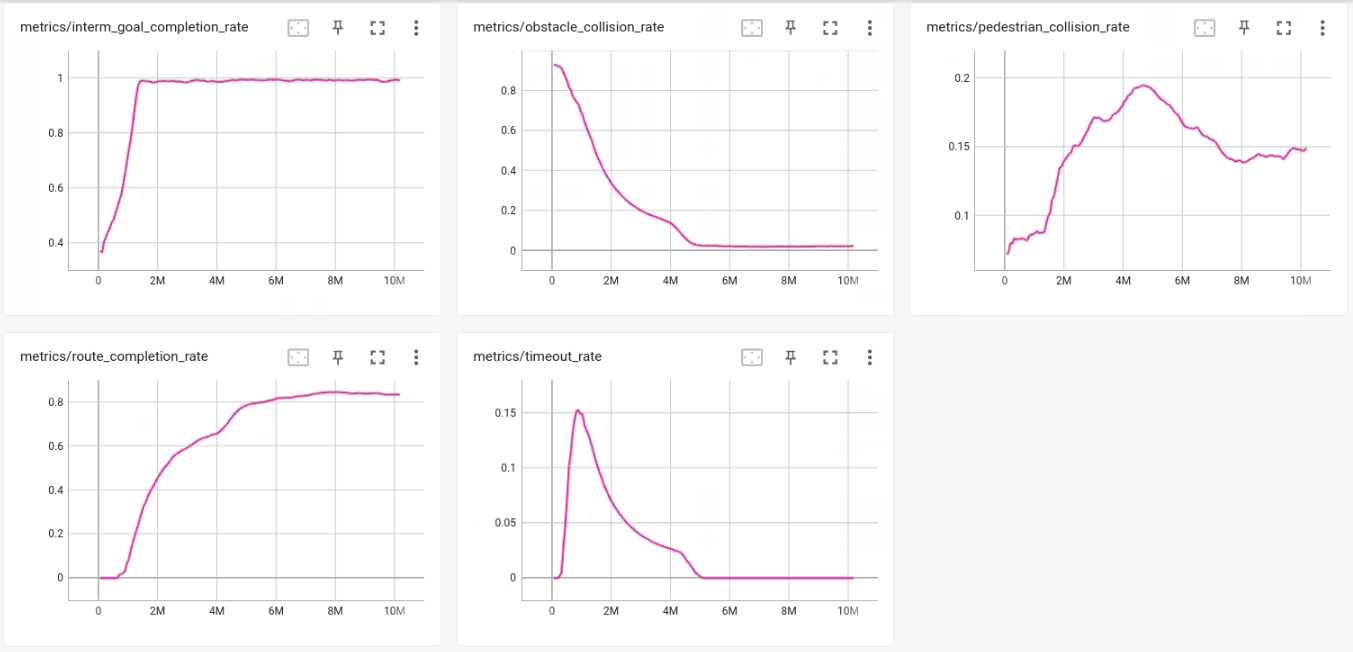
\includegraphics[width = 1.0\textwidth]{imgs/unfallraten_typisches_beispiel}
  \caption{Typischer Verlauf der Unfallmetriken während des Trainings. Zu sehen
  sind zeilenweise von rechts nach links die Komplettierungsrate von Wegpunkt
  zu Wegpunkt, die Kollisionsraten mit Fußgängern bzw. Hindernissen, die Rate
  komplettierter Routen und die Timeout-Rate. Auf x- und y-Achse sind jeweils die Zeit
  und die Rate zwischen 0 und 1 aufgetragen.}
  \label{fig:TypicalCollRates}
\end{figure}

Aufgrund der Stochastizität der erlernten Strategien unterliegen die Unfallmetriken
starken Schwankungen. Es genügen oftmals schon wenige, fehlerhafte Vorhersagen,
um einen Unfall herbeizuführen, der bei einer deterministischen Schätzung nicht
geschehen wäre. Daher werden zur Evaluation immer die geschätzten Mittelwerte für die
Aktuatoren statt der während des Trainings üblichen, normalverteilten Schätzungen
verwendet. Aufgrund der Notwendigkeit, die für die Modellaktualisierung benötigten
Trainingsdaten mit einer stochastischen Strategie zu sammeln, haben zur Trainingszeit
erhobene Unfallmetriken nur eine geringe Aussagekraft und dienen lediglich als grobe
Anhaltspunkte. Die folgenden Ergebnisse werden deshalb mit deterministisch
vorhergesagten Aktionen austrainierter Agenten ausgewertet. Je Auswertung fährt der
Agent 100 Routen, sodass die resultierenden Ergebnisse auf 1\% genau sind. Insbesondere
für die Bereiche $[0.00, 0.01]$ und $[0.99, 1.00]$ besteht daher keine Aussagekraft.
Dies stellt jedoch kein Problem dar, da die zu vergleichenden Ergebnisse ohnehin
keine entsprechende Qualität aufweisen.\\

Zur Evaluation werden alle erfolgreichen Trainingsläufe aus Tablelle \ref{tab:TrainingRuns}
betrachtet. Experiment 01 dient als Grundlinie für die ursprüngliche Umsetzung der
Trainingsumgebung durch Caruso et. al \cite{machines11020268} bezüglich Kartenmaterial
und Rewardstruktur.

\begin{table}[h]
\centering
\begin{tabular}{ |p{3cm}||c|c|c|c| }
 \hline
 Unfallmetrik vs. Trainingslauf & Completion & Obst. Coll. & Ped. Coll. & Timeout \\
 \hline \hline
 Experiment 01 & 0.08 & 0.00 & 0.00 & 0.92 \\ \hline
 Experiment 02 & 0.81 & 0.19 & 0.00 & 0.00 \\ \hline
 Experiment 03 & 0.05 & 0.00 & 0.00 & 0.95 \\ \hline
 Experiment 04 & 0.30 & 0.00 & 0.00 & 0.70 \\ \hline
 Experiment 05 & 0.14 & 0.00 & 0.00 & 0.86 \\ \hline
 Experiment 06 & 0.73 & 0.27 & 0.00 & 0.00 \\ \hline
 Experiment 07 & 1.00 & 0.00 & 0.00 & 0.00 \\ \hline
 Experiment 08 & 1.00 & 0.00 & 0.00 & 0.00 \\
 \hline
 \end{tabular}
 \caption{Auswertung der Unfallzahlen ohne Fußgänger}
 \label{tab:EvalNoPeds}
\end{table}

Wie in Tabelle \ref{tab:EvalNoPeds} zu sehen ist, wird zunächst zur Kontrolle eine Auswertung
ohne Fußgänger durchgeführt, um zu prüfen, ob die jeweilige Fahrsoftware statischen Hindernissen
ausweichen kann und die einfachere Aufgabe ohne bewegliche Hindernisse einwandfrei lösen kann.
Hier wäre eine Rate von 100\% zu erwarten, da die Problemstellung deutlich einfacher als mit
Fußgängern ist. Es zeigt sich aber, dass einige Agenten die Problemstellung nur unzureichend
lösen, was vielfältige Gründe haben kann. Beispielsweise
ist in der Live-Ansicht beobachtbar, dass die Agenten aus den Experimenten 02 bis 05 die Route
bis ans Ziel fahren, aber den letzten Wegpunkt meiden, weil sich dieser zu nah an einem Gebäude
befindet. Vermutlich ist ein entsprechendes Verhalten auf den Mangel an Engstellen
im Kartenmaterial zurückzuführen. Interessanterweise schneidet der mit einer komplexen
Rewardstruktur trainierte Agent in einer Umgebung ohne Fußgänger erstaunlich schlecht ab,
was nur schwer nachvollziehbar ist. Hingegen können die aus den Experimenten 07 und 08
resultierenden Agenten überzeugen, was vermutlich daran liegt, dass die Agenten
mit demselben Kartenmaterial trainiert wurden.\\

\begin{table}[h]
\centering
\begin{tabular}{ |p{3cm}||c|c|c|c| }
 \hline
 Unfallmetrik vs. Trainingslauf & Completion & Obst. Coll. & Ped. Coll. & Timeout \\
 \hline \hline
 Experiment 01 & 0.89 & 0.00 & 0.00 & 0.11 \\ \hline
 Experiment 02 & 0.59 & 0.13 & 0.28 & 0.00 \\ \hline
 Experiment 03 & 0.07 & 0.00 & 0.60 & 0.33 \\ \hline
 Experiment 04 & 0.38 & 0.06 & 0.02 & 0.54 \\ \hline
 Experiment 05 & 0.64 & 0.00 & 0.00 & 0.36 \\ \hline
 Experiment 06 & 0.18 & 0.25 & 0.57 & 0.00 \\ \hline
 Experiment 07 & 0.95 & 0.02 & 0.03 & 0.00 \\ \hline
 Experiment 08 & 0.93 & 0.01 & 0.06 & 0.00 \\
 \hline
\end{tabular}
\caption{Auswertung der Unfallzahlen mit Fußgängerdichte 0.02}
 \label{tab:EvalFewPeds}
\end{table}

In der zweiten Evaluation, deren Ergebnisse in Tabelle \ref{tab:EvalFewPeds} zu sehen sind,
werden die trainierten Agenten in einer Umgebung mit einer geringen Fußgängerdichte getestet.
Hierbei wird geprüft, ob die jeweilige Fahrsoftware vereinzelten, beweglichen Hindernissen
ausweichen kann und dabei nicht mit statischen Hindernissen Kollidiert. Es zeigt sich,
dass die Agenten mit kinematischem Fahrradmodell und einer verbesserten Sensorik besonders
gut abschneiden, da sie die Bewegungsdynamiken aus den Sensordaten extrahieren und somit
deren Bewegung einschätzen können, um adäquat auszuweichen. Hingegen weisen die Experimente
mit Differential Drive Kinematik und einer aus Standbildern bestehenden Sensorik deutlich
defensivere Verhaltensweisen auf, was auch im Live Debugging zu beobachten ist. Der Ansatz
mit alter Belohnungsstruktur und Kartenmaterial aus Experiment 01 schneidet gut ab,
was möglicherweise auf den Belohnungsterm zur Annäherungung an den nächsten Wegpunkt
zurückzuführen ist.\\

\begin{table}[h]
\centering
\begin{tabular}{ |p{3cm}||c|c|c|c| }
 \hline
 Unfallmetrik vs. Trainingslauf & Completion & Obst. Coll. & Ped. Coll. & Timeout \\
 \hline \hline
 Experiment 01 & 0.20 & 0.08 & 0.07 & 0.65 \\ \hline
 Experiment 02 & 0.16 & 0.11 & 0.73 & 0.00 \\ \hline
 Experiment 03 & 0.02 & 0.04 & 0.76 & 0.18 \\ \hline
 Experiment 04 & 0.59 & 0.07 & 0.11 & 0.23 \\ \hline
 Experiment 05 & 0.61 & 0.04 & 0.00 & 0.35 \\ \hline
 Experiment 06 & 0.01 & 0.20 & 0.79 & 0.00 \\ \hline
 Experiment 07 & 0.60 & 0.09 & 0.30 & 0.01 \\ \hline
 Experiment 08 & 0.51 & 0.13 & 0.35 & 0.01 \\
 \hline
\end{tabular}
\caption{Auswertung der Unfallzahlen mit Fußgängerdichte 0.08}
 \label{tab:EvalManyPeds}
\end{table}

In den letzten beiden Evaluationen, deren Ergebnisse in den Tabellen \ref{tab:EvalManyPeds}
und \ref{tab:EvalVeryCrowded} zu sehen sind, werden die trainierten Agenten in einer Umgebung
mit sehr dichtem Verkehr getestet. Hierbei steht die Unfallvermeidung, ohne Schäden an Personen,
Hindernissen und dem Fahrzeug zu verursachen im Vordergrund. Um die Aufgabe anspruchsvoller
zu gestalten, müssen die Agenten bewusst durch belebte Zonen hindurch fahren, was durch
entsprechend positionierte Wegpunkte erreicht wird. Die Schwierigkeit der Aufgabe besteht nun
darin, selbst bei dichtem Verkehr noch sicher Fortschritte erzielen zu können. Um die Aufgabe
überhaupt lösbar zu gestalten, weichen die Fußgänger dem Fahrzeug mittels \emph{Ped-Robot Force}
aus. Besonders hervorzuheben sind die Ergebnisse aus Experiment 05, wobei keine einzige
Kollision mit Fußgängern festzustellen ist. Der Agent kommt mit einer Ankunftsrate von
über 60\% am Routenziel an und wartet in fast allen weiteren Fällen ab. Die Ansätze
mit kinematischem Fahrradmodell und verbesserter Sensorik erreichen auch noch nennenswert
oft ihr Ziel, weisen jedoch eine offensive Fahrweise auf. Dies kann zum einen an der
Durchführung der Trainingsläufe bei weitaus geringerer Verkehrsdichte liegen.
Zum anderen ist auch denkbar, dass sich die Agenten zu sicher sind, die Dynamiken
der Fußgänger korrekt einschätzen zu können, was anschließend zu Unfällen führt.
Der mit komplexer Rewardstruktur trainierte Agent aus Experiment 01 kann nur schwer
Fortschritte erzielen, verursacht jedoch auch keine erhebliche Anzahl an Unfällen.

\begin{table}[h]
\centering
\begin{tabular}{ |p{3cm}||c|c|c|c| }
 \hline
 Unfallmetrik vs. Trainingslauf & Completion & Obst. Coll. & Ped. Coll. & Timeout \\
 \hline \hline
 Experiment 01 & 0.07 & 0.10 & 0.12 & 0.71 \\ \hline
 Experiment 02 & 0.10 & 0.18 & 0.72 & 0.00 \\ \hline
 Experiment 03 & 0.02 & 0.00 & 0.79 & 0.19 \\ \hline
 Experiment 04 & 0.39 & 0.10 & 0.20 & 0.31 \\ \hline
 Experiment 05 & 0.62 & 0.03 & 0.00 & 0.35 \\ \hline
 Experiment 06 & 0.00 & 0.17 & 0.83 & 0.00 \\ \hline
 Experiment 07 & 0.50 & 0.15 & 0.32 & 0.03 \\ \hline
 Experiment 08 & 0.33 & 0.14 & 0.52 & 0.01 \\
 \hline
\end{tabular}
\caption{Auswertung der Unfallzahlen mit Fußgängerdichte 0.10}
 \label{tab:EvalVeryCrowded}
\end{table}

\section{Vergleich der Ergebnisse}
Für einen fairen Vergleich werden die veröffentlichten Ergebnisse von Caruso et. al
\cite{machines11020268} herangezogen, da hier die meisten fachlichen und
konzeptionellen Überschneidungen bestehen und dieselben Unfallmetriken zur Auswertung
verwendet werden. Ihre Ergebnisse werden in Tabelle \ref{tab:EvalTriest}
zusammegefasst.\\

\begin{table}[h]
\centering
\begin{tabular}{ |p{3cm}||c|c|c|c| }
 \hline
 Unfallmetrik vs. Fußgängerdichte & Completion & Obst. Coll. & Ped. Coll. & Timeout \\
 \hline \hline
 0.00 / $m^2$ & 1.00 & 0.00 & 0.00 & 0.00 \\ \hline
 0.02 / $m^2$ & 0.87 & 0.00 & 0.13 & 0.00 \\ \hline
 0.08 / $m^2$ & 0.67 & 0.00 & 0.32 & 0.01 \\ \hline
 0.10 / $m^2$ & 0.52 & 0.01 & 0.47 & 0.00 \\ \hline
\end{tabular}
 \caption{Auswertung der Unfallzahlen von Caruso et. al \cite{machines11020268} mit A3C}
 \label{tab:EvalTriest}
\end{table}

Es zeigt sich, dass der Ansatz mit \emph{RobotSF} in seiner ursprünglichen Form zuverlässig
in Szenarien mit wenigen Fußgängern funktioniert und in etwa mit Experiment 07 vergleichbar
ist. Bei dichtem Verkehr weist die Fahrsoftware starke Schächen auf, da hohe Kollisionsraten
mit Fußgängern bestehen. Die defensive Strategie aus Experiment 05 erreicht ähnlich
gute Ankunftsraten, verursacht jedoch keine Kollisionen mit Fußgängern. Es kann also
von einer klaren Qualitätsverbesserung bei der Fahrsicherheit gesprochen werden.
Der Trainingsansatz, Agenten gezielt durch große Menschenmengen fahren zu lassen, scheint
vielversprechend. Ähnlich wie in Fan et. al \cite{fan2020distributed} könnte eine Kombination
einer defensiven und offensiven Fahrweise der Agenten aus Experiment 05 und 07 das Fahrverhalten
nochmals deutlich verbessern, indem bei wenig Verkehr die offensive und bei viel
Verkehr die defensive Fahrweise zum Einsatz kommt.\\

Da die Umsetzung einer Simulationsumgebung mit mehreren gleichzeitig agierenden Fahrzeugen
wie im Ansatz von \emph{Multi-Robot} zeitlich nicht mehr möglich war, ist ein Vergleich mit
Fan et. al \cite{fan2020distributed} nicht sinnvoll.
